% ************************** Panel **************************
% Use one of the following method:

% Method 1: SGS will send you a PDF file, you can insert it here directly.
%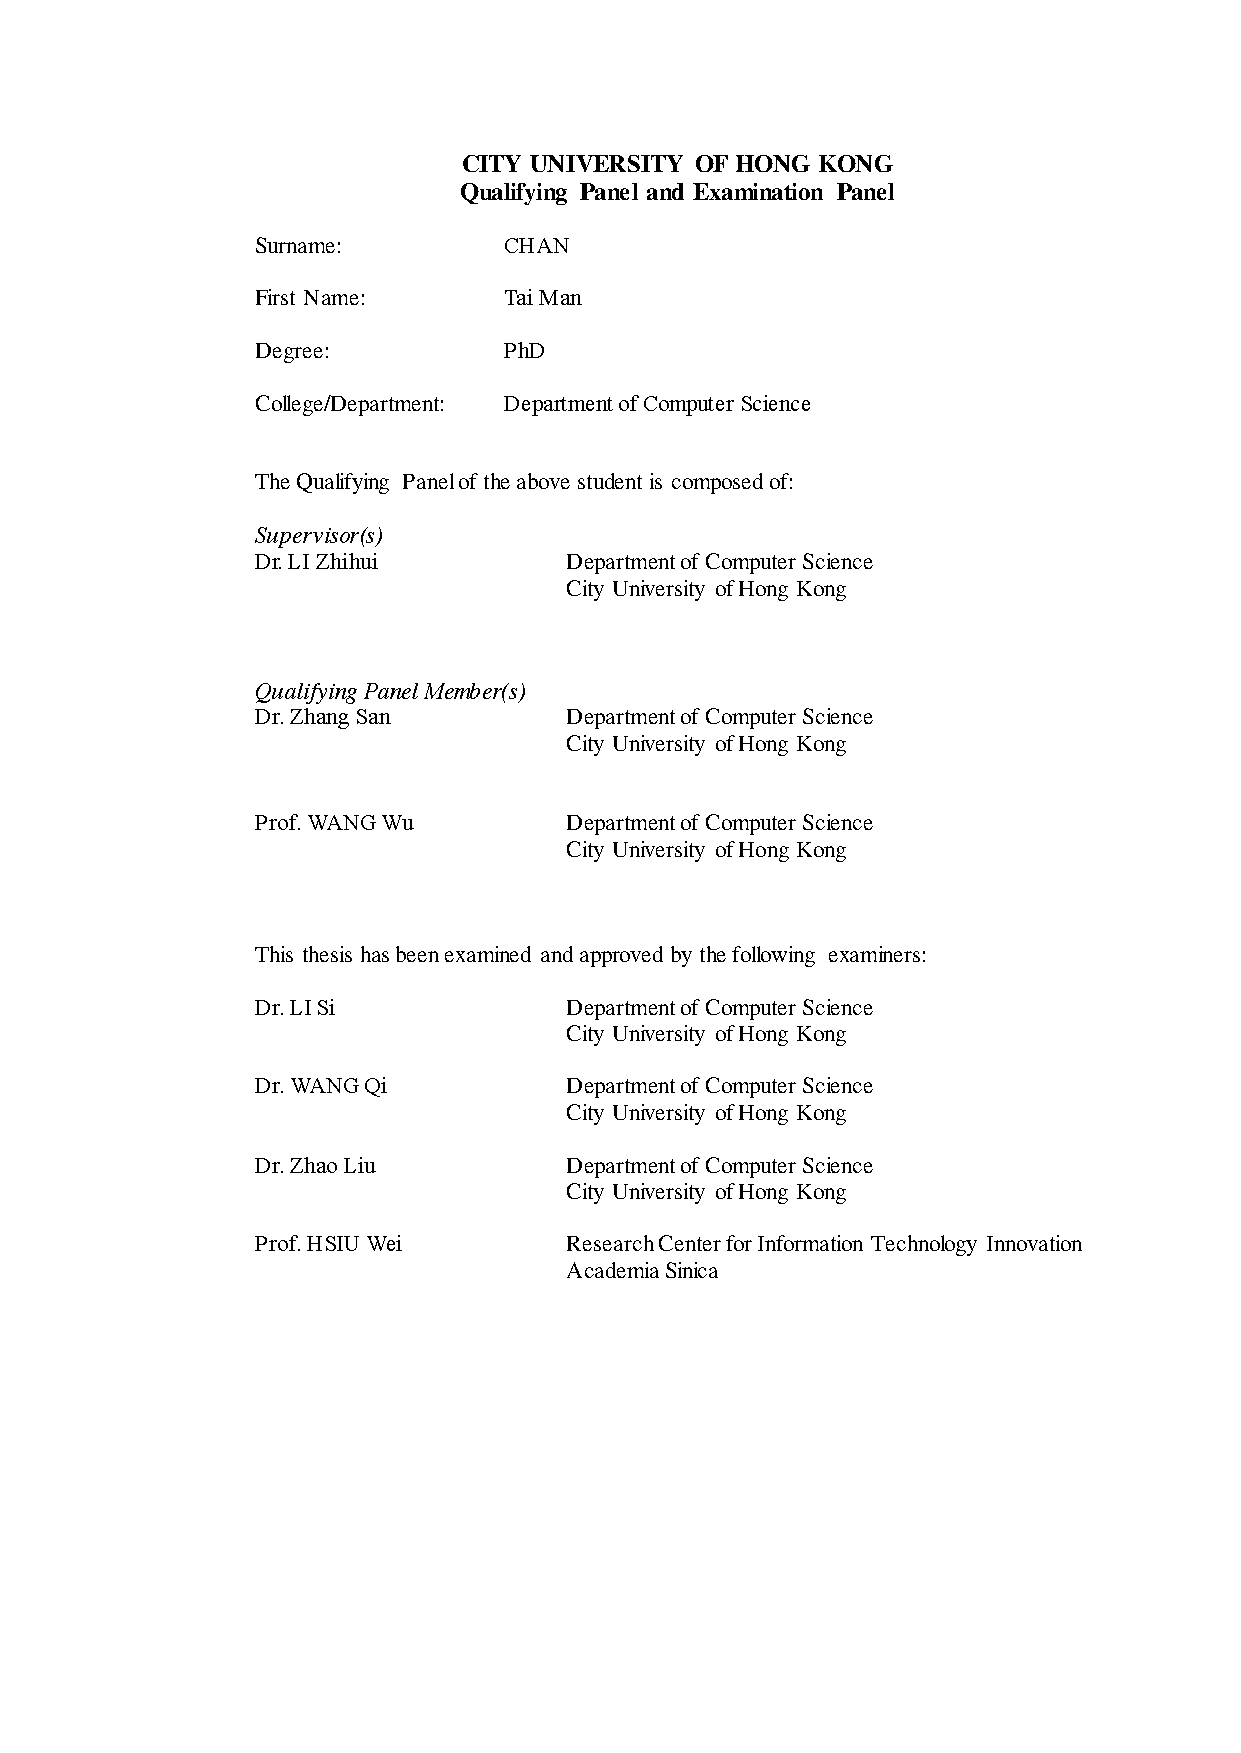
\includepdf[pagecommand={\thispagestyle{plain}}]{Front/qpsheet.pdf}

% Method 2:
% You may need to adjust the space to fit contents to one page
\begin{panel}

\begin{tabular}{p{40mm}p{80mm}}
Surname: & CHAN\tabularnewline
First Name: & Tai Man\tabularnewline
Degree: & PhD\tabularnewline
College/Department: & Department of Computer Science
\end{tabular}

\vspace{2em}

The Qualifying Panel of the above student is composed of:

\vspace{1em}

\begin{tabular}{p{50mm}p{80mm}}
\textit{Supervisor(s)} & \tabularnewline
Dr. SURNAME Name & Department of Computer Science\tabularnewline
 & City University of Hong Kong\\[1em]\tabularnewline

%\textit{Co-supervisor(s)} & \tabularnewline
%Name SURNAME & Department of ???\tabularnewline
% & City University of Hong Kong\\[.2em]\tabularnewline
 
\textit{Qualifying Panel Member(s)} & \tabularnewline
Prof. SURNAME Name & Department of Computer Science\tabularnewline
 & City University of Hong Kong\\[.2em]\tabularnewline

Dr. SURNAME Name & Department of Computer Science\tabularnewline
 & City University of Hong Kong\\[.2em]\tabularnewline
\end{tabular}

\vspace{2em}

This thesis has been examined and approved by the following examiners:
\vspace{1em}

\begin{tabular}{p{50mm}p{80mm}}
Prof. SURNAME Name & Department of Computer Science\tabularnewline
 & City University of Hong Kong\\[.2em]\tabularnewline

Dr. SURNAME Name & Department of Computer Science\tabularnewline
 & City University of Hong Kong\\[.2em]\tabularnewline

Prof. SURNAME Name & Department of Computer Science\tabularnewline
 & City University of Hong Kong\\[.2em]\tabularnewline

Dr. SURNAME Name & Department of Computer Science\tabularnewline
 & City University of Hong Kong\\[.2em]\tabularnewline
\end{tabular}

\end{panel}
